\section{Interpretação física do rotacional}
\begin{frame}
    \frametitle{Interpretação física do rotacional}
    \begin{itemize}
        \item A razão para o nome \textit{rotacional} é que o vetor rotacional está associado com rotações.
        \item Outra ocorre quando $F$ representa um campo de velocidade em mecânica dos fluidos.
        \item O rotacional de um campo de vetores que representa a velocidade de um fluido, está relacionado ao fenômeno de rotação do fluído. Existe uma relação entre rotacional e aspectos rotacionais do movimento.
    \end{itemize}
\end{frame}

\begin{frame}
    \frametitle{Interpretação física do rotacional}
    Seja $F$ um campo de vetores que representa o campo de velocidade de um fluido e consideramos uma partícula situada no ponto $\vec{F}$.
    \vspace{3mm}
    
    As particulas situadas num vizinhança deste ponto, tendem a rodar em torno do eixo que aponta na direção do $\text{\textit{rot}} \vec{F}(x,y,z)$, e o comprimento desse vetor rotacional é a medida de quão rápido as partículas se movem em torno desse eixo.
    
    \begin{figure}[h]
        \centering
        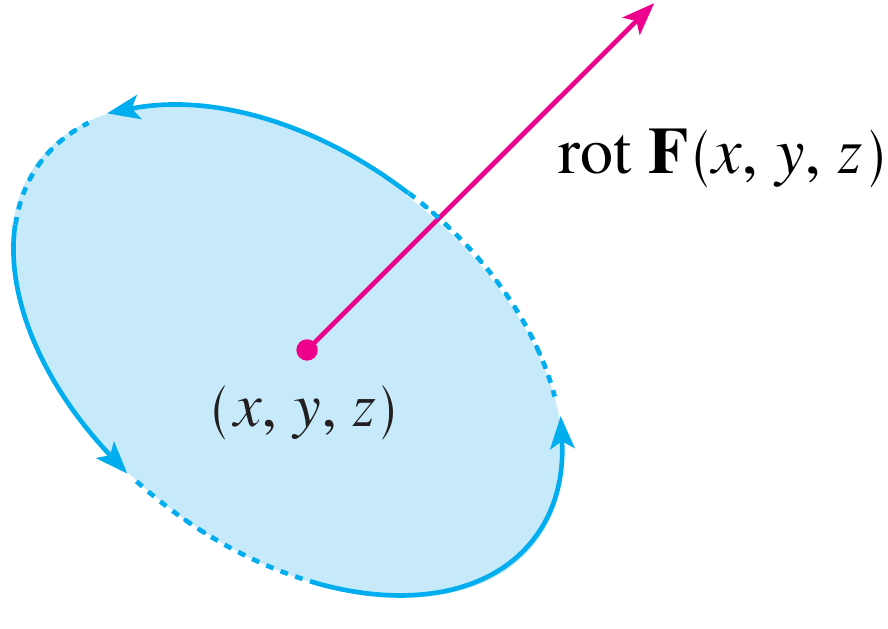
\includegraphics[scale=0.2]{img/rotacional.png}
    \end{figure}
\end{frame}

\begin{frame}
    \frametitle{Interpretação física do rotacional}
    \justifying
    Como já dito, o rotacional pode ter sua representação física relacionada à capacidade de giro que uma parte infinitesimal de um campo vetorial apresenta. Para auxiliar na visualização, vamos imaginar um campo vetorial qualquer, tomo como exemplo a função $F(x,y)=-y\vec{i}+x\vec{j}$.
    
    \begin{figure}[h]
        \centering
        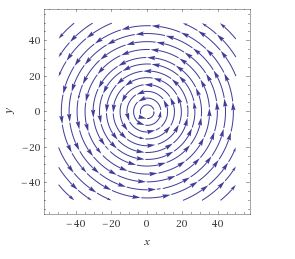
\includegraphics[scale=0.7]{img/Campo_Vetorial.jpg}
    \end{figure}
\end{frame}

\begin{frame}
    \frametitle{Interpretação física do rotacional}
    \justifying
    Então é colocado um disco dentro da água, e este disco tem um \textit{"Norte"}, que consiste no seu sentido de orientação. Ao ser colocado dentro do campo vetorial o disco começa a se movimentar de forma circular, acompanhando o deslocamento da água, mas sem mudar seu sentido e direção, mantendo seu \textit{"Norte"}. Este campo é dado como irrotacional.
    
    \begin{figure}[h]
        \centering
        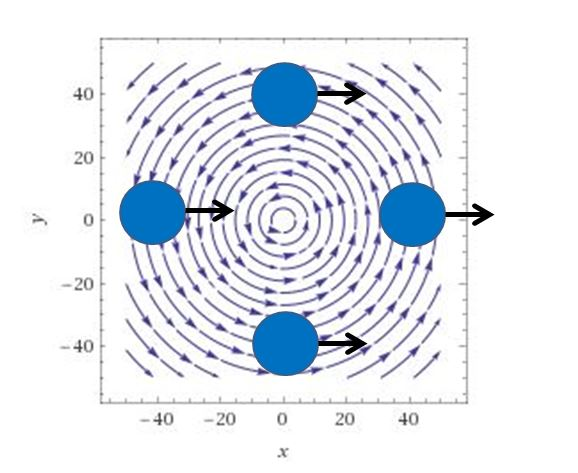
\includegraphics[scale=0.4]{img/Campo_Vetorial_com_Disco.jpg}
    \end{figure}
\end{frame}

\begin{frame}
    \frametitle{Interpretação física do rotacional}
    \justifying
    Agora imagine que outro disco é colocado dentro da água, só que desta vez, o centro do disco começa a se movimentar e girar em torno do seu prórpio eixo, ao longo do seu movimento, seu \textit{"Norte"} muda de sentido e direção. Esta capacidade do disco girar ao longo do movimento pode ser interpretada como o rotacional do campo vetorial.
    
    \begin{figure}[h]
        \centering
        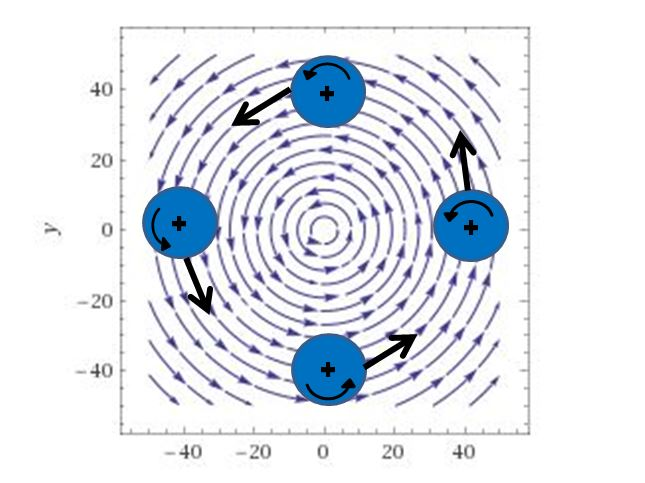
\includegraphics[scale=0.4]{img/Campo_Vetorial_com_Disco_Girando.jpg}
    \end{figure}
\end{frame}

\begin{frame}
    \frametitle{Interpretação física do rotacional}
    \justifying
    O rotacional pode ser obtido através da regra da mão direita, em que se posicionam os 4 dedos acompanhando o movimento de giro do disco, e por consequência, o polegar acaba apontando na direção do rotacional. No caso do disco, utilizando a regra, conclui-se que o rotacional está apontando para o eixo $\vec{k}$ positivo, isto é, para fora.
    
    \begin{figure}[h]
        \centering
        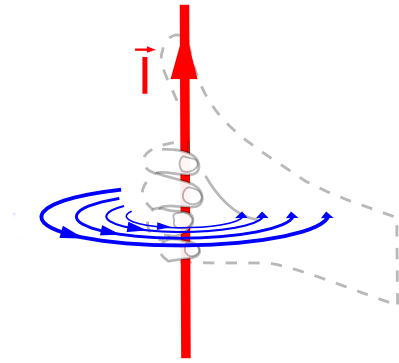
\includegraphics[scale=0.3]{img/Right_hand_rule.png}
    \end{figure}
\end{frame}

\begin{frame}
    \frametitle{Interpretação física do rotacional}
    \justifying
    Para o campo $F(x,y)$ dado, tem-se:
    
    \begin{displaymath}
        \nabla \times \vec{F} = \left| \begin{array}{ccc}
            \vec{i}                     & \vec{j}                     & \vec{k}                     \\[3mm]
            \frac{\partial}{\partial x} & \frac{\partial}{\partial y} & \frac{\partial}{\partial z} \\[3mm]
            -y                          & x                           & 0
        \end{array}\right|
    \end{displaymath}
    Calculando-se então o determinante:
    \begin{equation*}
        det = \left(
        \frac{\partial}{\partial y} \cdot 0 - \frac{\partial}{\partial z} \cdot x
        \right)\vec{i} + \left(
        \frac{\partial}{\partial z} \cdot (-y) - \frac{\partial}{\partial x} \cdot 0
        \right)\vec{j} + \left(
        \frac{\partial}{\partial x} \cdot x - \frac{\partial}{\partial x} \cdot (-y)
        \right)\vec{k}
    \end{equation*}
    Calculando as derivadas, tem-se então:
    \\[3mm]
    $det = (0-0)\vec{i}+(0-0)\vec{j}+(1+1)\vec{k}$
\end{frame}